% Preliminary report: Assignment 3, Benchmarking ANN search.
% Build from this directory: latexmk -pdf report.tex
% Every number below comes from results/full/ (tables/*.md, *.json).
\documentclass[10pt,a4paper]{article}
\usepackage[margin=1.8cm]{geometry}
\usepackage{graphicx}
\usepackage{booktabs}
\usepackage{amsmath}
\usepackage{hyperref}
\usepackage[font=small]{caption}
\usepackage{enumitem}
\setlist{nosep,leftmargin=*}
\graphicspath{{../results/full/figures/}}

\title{Benchmarking Approximate Nearest Neighbour Search\\\large CS4.406 Assignment 3 (preliminary draft)}
\author{Sohan Thummala}
\date{}

\begin{document}
\maketitle
\vspace{-2em}

\paragraph{Setup.}
Apple M2 (8 cores), 16\,GB RAM, macOS 26.6; Python 3.12.9, FAISS 1.15.1 (CPU), NumPy 2.5.4.
Datasets: SIFT-1M (128-d) and GloVe-100 (1.18M, 100-d, L2-normalised), both searched with
Euclidean distance. Tuning uses queries 0--4999; every reported number uses queries 5000--9999.
QPS is single-query, single-thread, median of 3 repeats. Searches return $k'=20$ so that
recall@10 can count ties at the 10th place as hits. \emph{Hypotheses:} both are recorded in
\texttt{README.md} rather than a separate \texttt{hypothesis.md}; the git history shows each
committed before its experiment (scaling: \texttt{213015d} before results in \texttt{7f15295};
drift: \texttt{0263641} before \texttt{5b6be69}).

\section{Exact baseline}
FAISS \texttt{IndexFlatL2} agrees with the stored neighbours on all 10{,}000 queries of both
datasets (tie-aware set comparison).

\begin{table}[h]\centering\small
\begin{tabular}{lrrrr}
\toprule
dataset & batch QPS (8 thr.) & single QPS (8 thr.) & batch QPS (1 thr.) & single QPS (1 thr.) \\
\midrule
SIFT  & 2265 & 58 & 1759 & 70 \\
GloVe & 1625 & 41 & 1637 & 62 \\
\bottomrule
\end{tabular}
\caption{Exact search on the 5000 report queries.}
\end{table}

\vspace{-1em}
Batching is 25--40$\times$ faster because a batch turns search into a matrix--matrix product
(BLAS GEMM): each block of base vectors is loaded from RAM once and reused against many queries
from cache. One query at a time is a matrix--vector product that streams the whole 512\,MB base
from memory for every query, so it is memory-bandwidth bound and pays per-call overhead.
Extra threads do not help single queries (they are slightly slower, from thread start-up per call).

\section{Three indexes}
Grid: HNSW $M\in\{16,32\}$, efConstruction 200, efSearch 32--512; IVF-Flat
$n_\text{list}=c\sqrt{n}$, $c\in\{1,4\}$, nprobe 1--128; IVF-PQ $c=4$, $m\in\{d/2,d/4\}$
sub-vectors of 8 bits, nprobe 1--256.

\begin{figure}[h]\centering
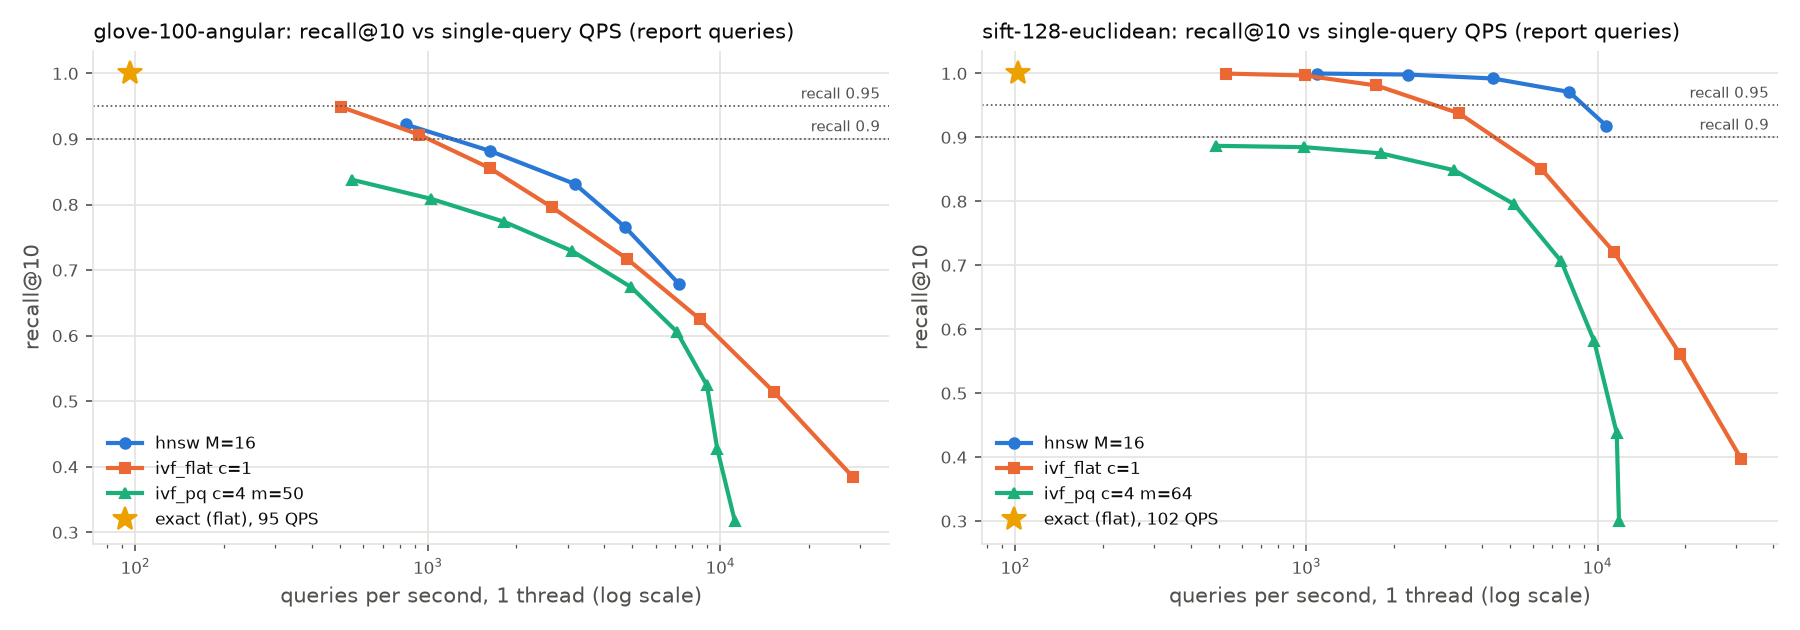
\includegraphics[width=\linewidth]{recall_vs_qps.png}
\vspace{-1.5em}
\caption{Recall@10 vs single-thread QPS. Solid: the build with the largest area under the curve;
dashed: other builds. Star: exact search.}
\end{figure}

\begin{table}[h]\centering\small
\begin{tabular}{llrlrl}
\toprule
dataset & index & QPS@0.90 & config & QPS@0.95 & config \\
\midrule
SIFT  & exact    & 70    & flat                   & 70   & flat \\
SIFT  & HNSW     & 13542 & $M$=16, ef=32          & 8190 & $M$=16, ef=64 \\
SIFT  & IVF-Flat & 6123  & $c$=4, nprobe=32       & 3578 & $c$=4, nprobe=64 \\
SIFT  & IVF-PQ   & --    & max recall 0.887       & --   & \\
GloVe & exact    & 62    & flat                   & 62   & flat \\
GloVe & HNSW     & 1371  & $M$=32, ef=256         & 707  & $M$=32, ef=512 \\
GloVe & IVF-Flat & 1066  & $c$=1, nprobe=64       & --   & max recall 0.949 \\
GloVe & IVF-PQ   & --    & max recall 0.838       & --   & \\
\bottomrule
\end{tabular}
\caption{Best QPS reaching each recall level (report queries).}
\end{table}

\begin{table}[h]\centering\small
\begin{tabular}{lllrrrr}
\toprule
dataset & index & config & recall & build s & size MB & bytes/vec \\
\midrule
SIFT  & HNSW     & $M$=16, ef=64            & 0.971 & 96.5  & 656.3 & 656.3 \\
SIFT  & IVF-Flat & $c$=4, nprobe=64         & 0.977 & 66.3  & 522.1 & 522.1 \\
SIFT  & IVF-PQ   & $m$=64, nprobe=256 (best) & 0.887 & 76.8  & 74.2  & 74.2 \\
GloVe & HNSW     & $M$=32, ef=512           & 0.965 & 236.6 & 795.5 & 672.2 \\
GloVe & IVF-Flat & $c$=1, nprobe=128 (best) & 0.949 & 6.5   & 483.3 & 408.4 \\
GloVe & IVF-PQ   & $m$=50, nprobe=256 (best) & 0.838 & 87.9  & 70.5  & 59.6 \\
\bottomrule
\end{tabular}
\caption{Build cost at recall 0.95 (or the highest-recall config where 0.95 was not reached).}
\end{table}

\vspace{-1em}
\textbf{Indexes that miss 0.95.} IVF-PQ plateaus (0.887 SIFT, 0.838 GloVe) even at nprobe=256:
once the right lists are scanned, the remaining error is in the PQ distance estimates, which
misorder close candidates; without exact re-ranking more probes cannot fix it. IVF-Flat on GloVe
stops at 0.949 because the sweep ends at nprobe=128 with $\sim$1088 lists: GloVe neighbours are
spread over more cells than SIFT's, so it needs more probes, not a different index.

\section{Experiment on standard data: scaling (SIFT)}
\begin{minipage}[t]{0.48\linewidth}\vspace{0pt}
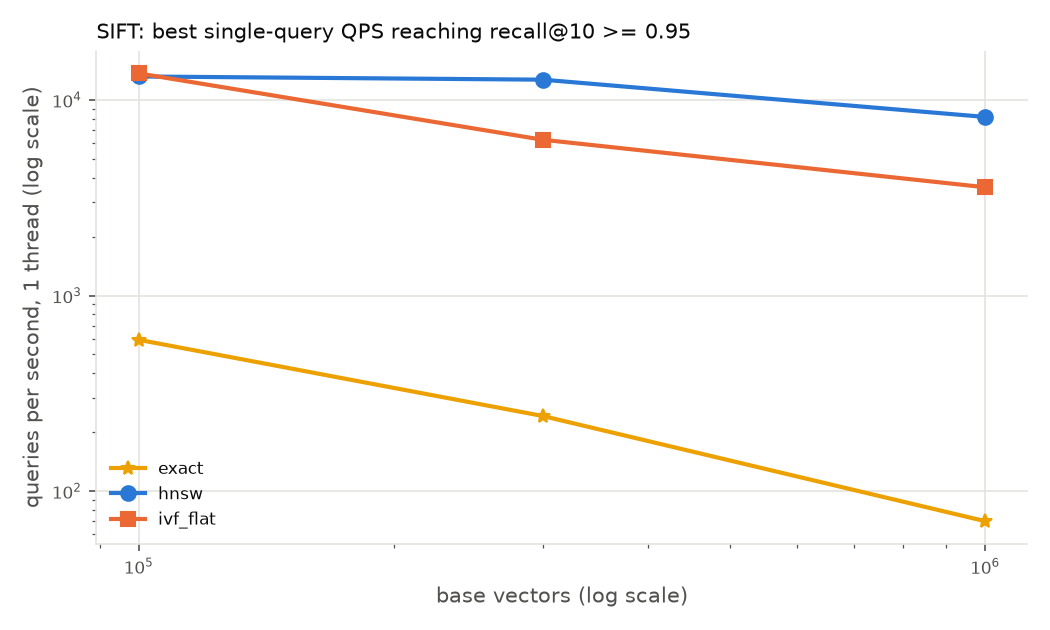
\includegraphics[width=\linewidth]{scaling_qps_at_0.95.png}
\end{minipage}\hfill
\begin{minipage}[t]{0.5\linewidth}\vspace{0pt}\small
\begin{tabular}{lrrr}
\toprule
$n$ & exact & HNSW & IVF-Flat \\
\midrule
100k & 593 & 13192 & 13678 \\
300k & 242 & 12703 & 6261 \\
1M   & 70  & 8190  & 3578 \\
\bottomrule
\end{tabular}

\smallskip
Best QPS at recall $\ge$ 0.95, every HNSW / IVF-Flat build tried at each size.
Exact cost grows linearly (10$\times$ data, 8.5$\times$ slower). IVF-Flat grows like
$\sqrt{n}$ (3.8$\times$): with $n_\text{list}\propto\sqrt{n}$ each list holds $\sim\sqrt{n}$
vectors and the needed nprobe also rises. HNSW grows slowest (1.6$\times$): greedy graph
search visits roughly $\log n$ layers/hops.
\end{minipage}

\smallskip
\textbf{Hypothesis check.} (1) Exact search scales worst: \emph{supported}. (2) HNSW and IVF-Flat
scale better than exact and HNSW beats IVF-Flat given the right parameters: \emph{supported};
they tie at 100k and HNSW leads by 2.0$\times$ at 300k and 2.3$\times$ at 1M.

\section{Experiment on own data: drift from a stale preprocessing step (SIFT, 300k base)}
\textbf{What changed.} A preprocessing change that the index was not rebuilt for. Two kinds,
never combined, each with three strengths plus the unchanged control (clean):
mean shift (add $c\in\{5,10,15\}$ to every coordinate) and pairwise rotation (rotate dimension
pairs $(0,1),(2,3),\dots$ by $2^\circ,3^\circ,5^\circ$). \emph{Stale}: index on the original base,
transformed queries. \emph{Rebuilt}: base and queries transformed, index rebuilt.
Two recalls: \emph{own} (vs exact neighbours of the transformed query in the indexed base) and
\emph{original} (vs neighbours of the original query in the original base). The transforms are
deterministic, so every run produces the same data.

\begin{figure}[h]\centering
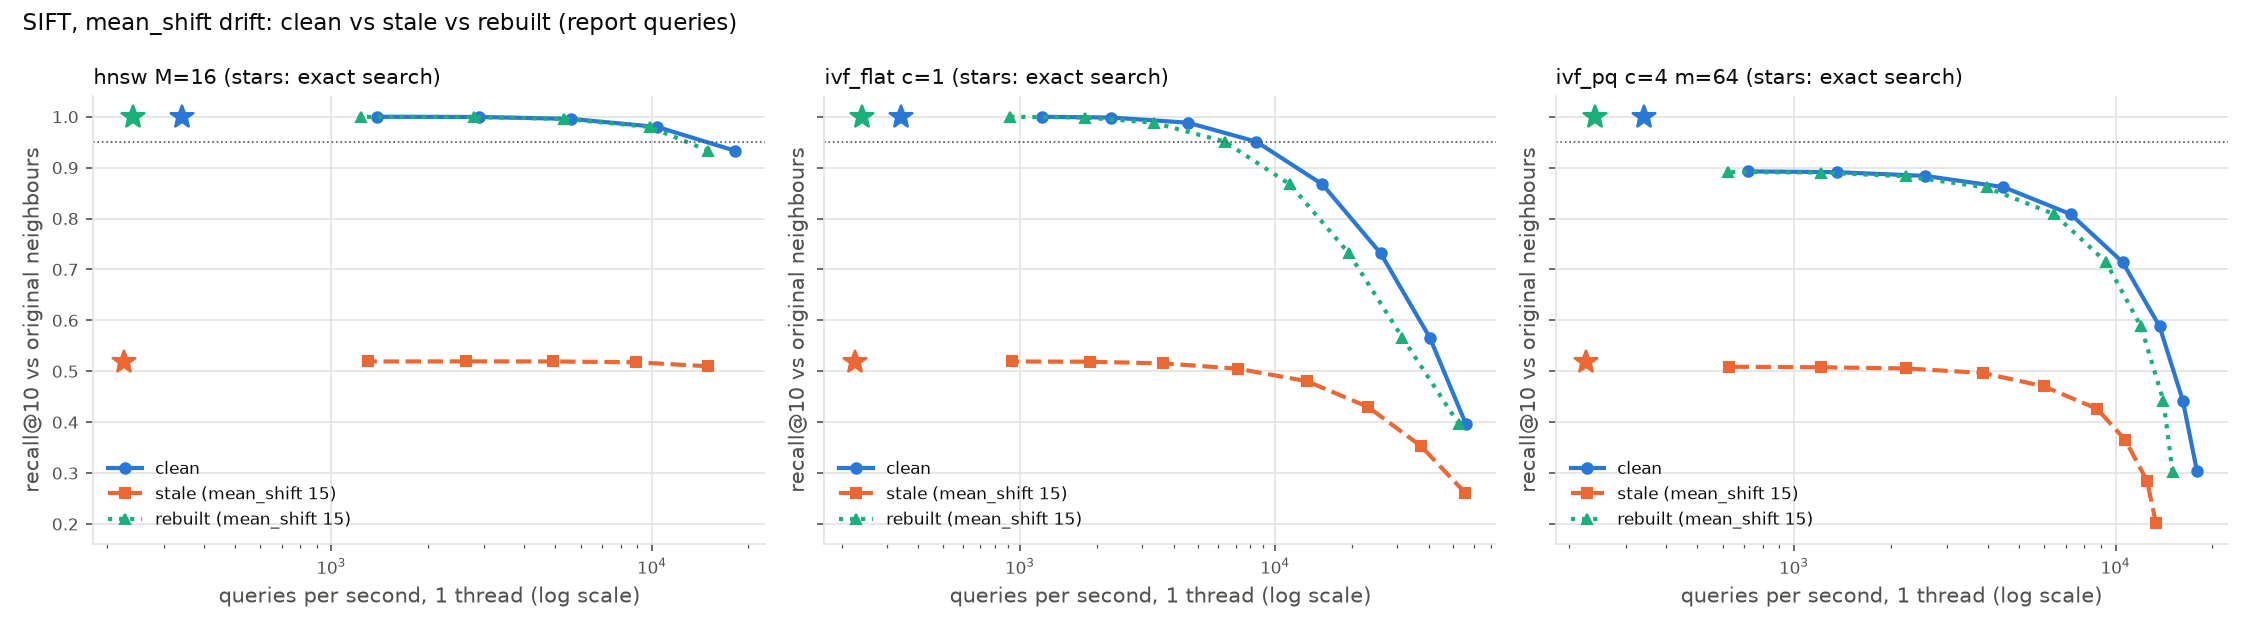
\includegraphics[width=\linewidth]{drift_mean_shift.png}
\vspace{-1.5em}
\caption{Mean shift $c=15$: clean, stale and rebuilt curves of the best build per index.}
\end{figure}

\begin{table}[h]\centering\small
\begin{tabular}{lrrrr|rrr}
\toprule
& \multicolumn{4}{c|}{stale $-$ clean, recall (original), top config} & \multicolumn{3}{c}{worst stale $-$ clean, recall (own)} \\
setting & exact & HNSW & IVF-Flat & IVF-PQ & HNSW & IVF-Flat & IVF-PQ \\
\midrule
shift 5    & $-0.170$ & $-0.170$ & $-0.170$ & $-0.093$ & $-0.006$ & $-0.020$ & $-0.018$ \\
shift 10   & $-0.329$ & $-0.328$ & $-0.329$ & $-0.237$ & $-0.017$ & $-0.048$ & $-0.044$ \\
shift 15   & $-0.481$ & $-0.480$ & $-0.481$ & $-0.384$ & $-0.033$ & $-0.078$ & $-0.073$ \\
rotate 2$^\circ$ & $-0.080$ & $-0.080$ & $-0.080$ & $-0.027$ & $-0.001$ & $-0.003$ & $-0.004$ \\
rotate 3$^\circ$ & $-0.118$ & $-0.118$ & $-0.118$ & $-0.050$ & $-0.001$ & $-0.006$ & $-0.005$ \\
rotate 5$^\circ$ & $-0.188$ & $-0.187$ & $-0.188$ & $-0.105$ & $-0.004$ & $-0.010$ & $-0.009$ \\
\bottomrule
\end{tabular}
\caption{Recall drops. Rebuilt is within $\pm0.003$ of clean for every config.}
\end{table}

\vspace{-1em}
\textbf{What happened.} Stale recall against the original neighbours falls with drift strength,
by the \emph{same amount for HNSW, IVF-Flat and exact search}: exact, HNSW and IVF-Flat all lose
their 0.95 configs at the weakest setting of both kinds. Recall against the transformed query's
own exact neighbours barely moves (worst $-0.08$, IVF at low nprobe and $c=15$). Rebuilding
recovers everything.

\textbf{Mechanism.} The loss is in the data, not the index. For a shift,
$\lVert q+c\mathbf{1}-x\rVert^2=\lVert q-x\rVert^2+2c\,\mathbf{1}^\top(q-x)+c^2d$: the middle term
re-ranks base points by their coordinate sum, so the true neighbour set itself changes and even
exact search returns the ``wrong'' answer. A rotation of only the query likewise moves it
relative to a fixed base. Rebuilding applies the same isometry (translation or rotation) to both
sides, so all distances are preserved and clean recall returns. The small own-recall loss in IVF
comes from coarse assignment: the shifted query lies off the data and closer to cell boundaries,
so a few probes pick worse lists; HNSW's greedy walk is less sensitive.

\textbf{Hypothesis check.} (1) Degradation against ground truth but similar to exact:
\emph{supported}. (2) QPS unchanged: \emph{mostly supported}; medians move 10--30\% with no
consistent direction, which is run-to-run noise. (3) IVF-PQ degrades most, IVF-Flat least:
\emph{not supported}; IVF-PQ's own-recall loss is no larger than IVF-Flat's and its
original-recall drop is \emph{smaller} only because it starts lower (0.893).

\textbf{Not tested.} Adding drifted vectors to an existing index (only queries drift);
retraining only the IVF coarse quantizer; drift on GloVe; scaling or normalisation changes.

\section{Discussion}
\textbf{Q1. Fastest at recall 0.95.} HNSW on both: 8190 QPS on SIFT (2.3$\times$ IVF-Flat) and
707 on GloVe (the only ANN index to reach 0.95). The winner does not change, but GloVe is
$\sim$11$\times$ slower: its neighbourhoods are less distinct (lower relative contrast), so HNSW
needs $M=32$ and ef=512 and IVF must probe many more lists.

\textbf{Q2. Build cost and memory.} HNSW is the costliest to build (96\,s SIFT, 237\,s GloVe)
and largest (656--672 B/vector: raw floats plus $2M$ graph links on layer 0). IVF-Flat is
cheaper (6.5--66\,s for k-means) at raw size plus ids. IVF-PQ stores 60--74 B/vector,
7--9$\times$ less, but its quantised distances cap recall at 0.84--0.89 and it is not even faster
at its best recall (456 QPS on SIFT), since high nprobe is needed to approach the cap.

\textbf{Q3. What the experiments imply.} Headline numbers hold only for the size and the query
distribution they were measured on. IVF-Flat matches HNSW at 100k but is 2.3$\times$ slower at
1M, so small-scale benchmarks mislead. Under a stale preprocessing step, recall measured against
the index's own exact search stays near 1 while real recall drops by up to 0.48: an internal
recall check cannot detect the problem.

\textbf{Q4. 150k or 10M vectors, 100\,ms, 16\,GB.} At 150k, exact single-thread search takes
$\sim$2.2\,ms (between 1.6\,ms at 100k and 4.1\,ms at 300k) and the vectors need 77\,MB: use
exact search, which gives perfect recall and no build. At 10M, exact scales to $\sim$144\,ms per
query (14.4\,ms at 1M $\times$10), over budget, and raw floats need 5.1\,GB. Use HNSW, $M=16$
($\sim$6.6\,GB including links, fits), with efSearch re-tuned on held-out queries at the new size
(64--128), because recall falls at fixed ef as $n$ grows. IVF-Flat ($c=4$) is a cheaper-to-build
fallback. These are extrapolations; 10M was not run.

\textbf{Q5. Ways this benchmark could mislead.} (a) \emph{Timing noise and overhead}: QPS on one
laptop varies 10--30\% between runs (seen on repeated clean measurements in the drift
experiment), and Python call overhead is a larger share for fast indexes. Medians of 3 reduce
this; overhead was not measured separately. (b) \emph{In-distribution queries}: queries come
from the same distribution as the base. The drift experiment tested this and showed real recall
can fall far below the headline number.

\end{document}
